\documentclass[letter,11pt]{article}

\usepackage[spanish,es-nodecimaldot]{babel}
\usepackage[utf8]{inputenc}

\usepackage{lmodern}
\usepackage[T1]{fontenc}
\usepackage{textcomp}

\usepackage{framed}
\usepackage[svgnames]{xcolor}
\colorlet{shadecolor}{Gainsboro!50}

\usepackage{enumitem}
\usepackage{graphicx}
\usepackage{pstricks}

\usepackage{anysize}
\marginsize{3cm}{2cm}{2cm}{3cm}

\usepackage{siunitx}
\usepackage{amsmath}
\usepackage{array}
\usepackage{alltt}

\usepackage{fancyhdr}
\usepackage{lastpage}
\pagestyle{fancy}
\fancyhf{}
\fancyhead[LE,RO]{Termodinámica}
\fancyfoot[CO,CE]{\thepage\ de \pageref{LastPage}}

\special{papersize=215.9mm,279.4mm}

\usepackage[
    pdfauthor={Carlos Eduardo Caballero Burgoa},%
    pdftitle={Termodinámica},%
    pdfsubject={Tarea 01},%
    colorlinks,%
    citecolor=black,%
    filecolor=black,%
    linkcolor=black,%
    urlcolor=black,
    breaklinks]{hyperref}
\usepackage{breakurl}

\newcommand{\blankpage}{
\newpage
\thispagestyle{empty}
\mbox{}
\newpage
}

\renewcommand{\arraystretch}{1.2}

\begin{document}

\begin{center}
    {\Large \bf{\underline{Tarea \#01}}}
\end{center}
\vspace{0.5cm}

\begin{enumerate}
\item \textbf{Hallar la presión atmosférica en \emph{Santa Cruz},
\emph{Cochabamba} y \emph{La Paz}.}

La presión atmosférica es el peso de la columna de aire que hay sobre cualquier
punto o lugar de la tierra y es por tanto el peso por unidad de superficie.

Cuanto mayor es la altura, menor es la presión atmosférica y cuanto menor es la
altura y más se acerque a nivel del mar, mayor será la presión.

\begin{center}
    \begin{tabular}{|>{\centering}m{3.0cm}<{\centering}|
                    |>{\centering}m{3.0cm}<{\centering}
                    |>{\centering}m{3.0cm}<{\centering}
                    |>{\centering}m{3.0cm}<{\centering}|}
    \hline
    \textbf{Ciudad} & 
    \textbf{Altitud (m.s.n.m.)} & 
    \textbf{Temperatura promedio $^\circ$C} & 
    \textbf{Presión (atm)} \tabularnewline \hline
    \hline
    La Paz     & 3650 & 13.0 & 0.647 \tabularnewline \hline
    Cochabamba & 2574 & 18.6 & 0.739 \tabularnewline \hline
    Santa Cruz &  400 & 24.6 & 0.947 \tabularnewline \hline
    \end{tabular}
\end{center}

\item \textbf{Cuál es la densidad del aire en \emph{Cochabamba}.}

Está comprobado que la mayor densidad de aire está al nivel del mar, en el que
el estándar es de $1.225\,[kg/m^3]$, entonces, a mayor altura, menor será la
densidad del aire.

En el caso de \emph{Cochabamba}, la ciudad a una altura de $2558\,[msnm]$
tendría una densidad del aire de $0,713\,[kg/m^3]$.

\item \textbf{Cuál es la temperatura ambiente en \emph{Cochabamba}.}

En \emph{Cochabamba}, los veranos son cortos, calurosos y mayormente nublados;
los inviernos son cortos, frescos y mayormente despejados y está seco durante
todo el año. Durante el transcurso del año, la temperatura generalmente varía de
$4 ^\circ C$ a $26 ^\circ C$ y rara vez baja a menos de $1 ^\circ C$ o sube a
más de $29 ^\circ C$.

\begin{figure}[!h]
\centering
\includegraphics[scale=0.68]{resources/fig1.eps}
\end{figure}

\item \textbf{Cuál es la temperatura de ebullición en \emph{Cochabamba}.}

El punto de ebullición de un líquido a $1 [atm]$ - $760 [mmHg]$, se conoce punto
de ebullición normal.

La temperatura de ebullición se ve afectada por los cambios en la presión
atmosférica debidos a las variaciones en la altura. A medida que un sitio se
encuentra más elevado sobre el nivel del mar, la temperatura de ebullición se
hace menor.

Para el calculo de la temperatura de ebullición se realizan los siguientes
cálculos:

\begin{enumerate}
\item Calcular la diferencia de presión atmosférica.

\begin{equation*}
\Delta P = P_{atm} \text{(nivel del mar)} - P_{atm} \text{(Cochabamba)}
\end{equation*}
\begin{equation*}
\Delta P = 760 [mmHg] - 561.64 [mmHg] = 198.36 [mmHg]
\end{equation*}

\item Se calcula el factor de corrección de la temperatura por cambio en la
presión atmosférica, con la siguiente ecuación:

\begin{equation*}
F_C = \frac{\Delta P * (\Delta T * \Delta P)}{10 [mmHg]}
\end{equation*}

Para el agua el factor de corrección por cada $10 [mmHg]$ es igual a: $0.370$.

Por tanto:

\begin{equation*}
F_C = 198.36 [mmHg] * \frac{0.370}{10 [mmHg]} = 7.34 ^\circ C
\end{equation*}

\item Se obtiene la temperatura de ebullición corregida:

\begin{equation*}
T_{eb} = 100 ^\circ C - 7.34 ^\circ C = 92.66 ^\circ C
\end{equation*}

\end{enumerate}

\end{enumerate}

\begin{thebibliography}{99}

\bibitem{SAILANDTRIP} Presión atmosférica; ¿Qué es y cómo se mide?\\
Extraído el 16 de Marzo del 2022, de:\\
\url{https://sailandtrip.com/presion-atmosferica/}
 
\bibitem{SLIDESHARE} Presión atmosférica\\
Extraído el 16 de Marzo del 2022, de:\\
\url{https://es.slideshare.net/sleven00/presion-atmosferica-134784932}

\bibitem{INE} Bolivia - Temperatura media por ciudad capital, según año y mes, 1990 - 2022\\
Extraído el 16 de Marzo del 2022, de:\\
\url{https://nube.ine.gob.bo/index.php/s/PDY4fnsFeSYKtRi/download}

\bibitem{TIEMPOS} Ciclismo ¿Por qué Cochabamba es la nueva sede para romper récords de pista?\\
Extraído el 16 de Marzo del 2022, de:\\
\url{https://www.lostiempos.com/deportes/multideportivo/20190929/ciclismo-que-cochabamba-es-nueva-sede-romper-records-pista}

\bibitem{WEATHERSPARK} El clima y el tiempo promedio en todo el año en Cochabamba\\
Extraído el 16 de Marzo del 2022, de:\\
\url{https://es.weatherspark.com/y/27676/Clima-promedio-en-Cochabamba-Bolivia-durante-todo-el-año}

\bibitem{SGPWE} Temperatura de ebullición y presión de vapor\\
Extraído el 16 de Marzo del 2022, de:\\
\url{http://sgpwe.izt.uam.mx/files/users/uami/acym/punto_de_ebullicion_correccion}

\end{thebibliography}

\end{document}

